\documentclass[
	12pt,				% tamanho da fonte
	openright,			% capítulos começam em pág ímpar (insere página vazia caso preciso)
	oneside,			% para impressão em recto e verso. Oposto a oneside
	a4paper,			% tamanho do papel. 
	english,			% idioma adicional para hifenização
	french,				% idioma adicional para hifenização
	spanish,			% idioma adicional para hifenização
	brazil				% o último idioma é o principal do documento
	]{abntex2}

\usepackage{lmodern}			% Usa a fonte Latin Modern			
\usepackage[T1]{fontenc}		% Selecao de codigos de fonte.
\usepackage[utf8]{inputenc}		% Codificacao do documento (conversão automática dos acentos)
\usepackage{indentfirst}		% Indenta o primeiro parágrafo de cada seção.
\usepackage{color}				% Controle das cores
\usepackage{graphicx}			% Inclusão de gráficos
\usepackage{microtype} 			% para melhorias de justificação
\usepackage{transparent}
\usepackage{eso-pic}
\usepackage{amsthm,amsfonts}
\usepackage{float}
\usepackage{multirow}
\usepackage[table,xcdraw]{xcolor}
\usepackage{longtable}
\usepackage{lipsum}				% para geração de dummy text
%\usepackage[brazilian,hyperpageref]{backref}	 % Paginas com as citações na bibl
\usepackage[alf]{abntex2cite}	% Citações padrão ABNT
\usepackage{xcolor}
\usepackage{scalefnt}
\usepackage{subfig}
\usepackage{lscape}
\usepackage[font=small]{caption}     %% make caption in normal size
\usepackage{etoolbox}
\AtBeginEnvironment{longtabu}{\footnotesize}{}{}   %% change all longtabu content to foot note size

\definecolor{verde}{rgb}{0,0.5,0}
\usepackage{listings}
%\lstset{
%  language=C++,
%  basicstyle=\ttfamily\small,
%  keywordstyle=\color{blue},
%  stringstyle=\color{verde},
%  commentstyle=\color{red},
%  extendedchars=true,
%  showspaces=false,
%  showstringspaces=false,
%  numbers=left,
%  numberstyle=\tiny,
%  breaklines=true,
%  backgroundcolor=\color{green!10},
%  breakautoindent=true,
%  captionpos=b,
%  xleftmargin=0pt,
%}


\titulo{Projeto de Desenvolvimento de Produto\\Filtro de Água para Pets}
\autor{Caio Henrique Silva Souza 99131\\Eduardo Favoretto Vale Bom 108139\\Gabriel Rodrigues Munhoz 106802\\João Vítor Batistão 108074}
\local{Maringá, PR}
\data{10.03.2022}
\orientador{}
\coorientador{}
\instituicao{%
  Universidade Estadual de Maringá - UEM
  \par
  Departamento de Engenharia de Produção - DEP}
\tipotrabalho{Tese (Doutorado)}
\preambulo{}

\definecolor{blue}{RGB}{41,5,195}

\makeatletter
\hypersetup{
     	%pagebackref=true,
	pdftitle={\@title}, 
	pdfauthor={\@author},
    	pdfsubject={\imprimirpreambulo},
	pdfcreator={LaTeX with abnTeX2},
	pdfkeywords={abnt}{latex}{abntex}{abntex2}{trabalho acadêmico}, 
	colorlinks=true,       		% false: boxed links; true: colored links
    	linkcolor=black,          	% color of internal links
    	citecolor=blue,        		% color of links to bibliography
    	filecolor=magenta,      		% color of file links
	urlcolor=blue,
	bookmarksdepth=4
}

\setlength{\parindent}{1.3cm}

\setlength{\parskip}{0.2cm}  % tente também \onelineskip

\makeindex

%\usepackage{fancyhdr}
%\fancyhead{}
%\fancyfoot{}
%\lhead{Processo Agroindustrial de Processamento de Cacau}
%\rhead{Processo Agroindustrial de Processamento de Cacau}

\AddToShipoutPicture{
\put(0,0){
\parbox[b][\paperheight]{\paperwidth}{%
\vfill
\centering
{\transparent{0.1}\includegraphics[scale=1.4]{../../Pictures/logoUEM.jpg}    }%
\vfill}}}



%\graphicspath{{../Pictures}}
\begin{document}

\begin{minipage}[c][0cm][c]{0cm} % a primeira minipágina tem uma altura de 1.5cm e uma largura de 3cm.

\centering


\includegraphics[scale=0.45]{../../Pictures/uem-modelo-04.png}  
\end{minipage}

\selectlanguage{brazil}

\frenchspacing 

% \pretextual

\imprimircapa


% ---
% RESUMOS
% ---

%\setlength{\absparsep}{18pt} % ajusta o espaçamento dos parágrafos do resumo
%\begin{resumo}
 
 
% \textbf{Palavras-chave}: latex. abntex. editoração de texto.
%\end{resumo}


% ---
% inserir o sumario
% ---
\pdfbookmark[0]{\contentsname}{toc}
\tableofcontents*
\cleardoublepage

% ----------------------------------------------------------
% ELEMENTOS TEXTUAIS
% ----------------------------------------------------------
\textual

\chapter{Introdução}
%\pagestyle{fancy}

\section{Contextualização do Tema}

O desenvolvimento de produtos é um setor que abrange diversas atividades, e todas
com notória importância. Para conseguir atingir o sucesso em um projeto é necessária
muita dedicação, planejamento e estudo de mercado.

O PDP, como é conhecido o Projeto de Desenvolvimento de Produto, é definido como sendo a transformação de necessidades do mercado em produtos ou serviços. O projeto pode ter caráter mais radical ou mais conservador, de acordo com a inovação presente no produto que está sendo desenvolvido, contudo, todos eles são únicos e possuem incertezas. \cite{rozenfeld}

Em uma empresa o PDP deve sempre estar alinhado com o Plano Estratégico de Negócios (PEN), pois com esse alinhamento a companhia consegue atingir suas metas de longo prazo e seus objetivos mais importantes. Entre esses surge o PEP, que é o Plano Estratégico de Produtos, o qual é de grande importância para a empresa, já que sempre tem o objetivo de manter um portfólio eficiente e muito lucrativo. \cite{rozenfeld}

Com tantas atividades e planejamentos, a empresa necessita de um processo de referência para que o PDP sempre ocorra de maneira padronizada e consiga abranger tudo, sem o esquecimento de etapas importantes. Para isso há o modelo de referência criado por Rozenfeld, que serve como um guia padrão, no entanto as empresas fazem suas adaptações de acordo com as necessidades de cada projeto. \cite{rozenfeld}

Esse modelo de referência é composto por 3 etapas: Pré-desenvolvimento, Desenvolvimento e Pós-desenvolvimento. A primeira etapa compõe o planejamento do projeto em si e o planejamento e revisão dos produtos da empresa, é possível observar revisões do PEN nessa etapa e também um alinhamento grande com o PEP. Dessa forma, a empresa sempre consegue projetar novos produtos de acordo com a estratégia de longo prazo da empresa. Na segunda etapa, ocorrem as formulações dos projetos informacional, conceitual e detalhado, além da preparação da linha de produção para receber o novo produto e o planejamento e execução do lançamento do produto. A fase de desenvolvimento é onde acontece a transformação da ideia em algo real. Já na etapa de pós-desenvolvimento ocorre o acompanhamento do produto já lançado e a possível descontinuação do mesmo. \cite{rozenfeld}

De fato, o desenvolvimento de um novo produto ou serviço é algo complexo que deve ser analisado com calma e deve ser muito bem planejado. A quantidade de informações que deve ser compilada para que um produto seja bem sucedido é proporcional à inovação presente nele e a utilização de diversos tipos de ferramentas para mapear e conseguir essas informações é de suma importância. 

Com isso, neste trabalho será realizado um Projeto de Desenvolvimento de Produto, composto por todas suas fases e uma grande variedade de ferramentas para que seja possível visualizar e entender a complexidade desse processo. O trabalho será de cunho mais explicativo utilizando uma empresa teórica para apresentação das etapas e as ferramentas mais utilizadas em cada uma delas.  


\section{Objetivos}

\subsection{Objetivo Geral}

O objetivo geral do trabalho é apresentar e praticar todas as etapas que englobam o desenvolvimento de um produto físico, montável e duŕavel a partir de uma empresa fictícia. Dessa forma, será utilizado um exemplo de um produto inovador para demonstrar como ocorrem as etapas de desenvolvimento, desde a escolha do projeto até a finalização e prototipagem.

\subsection{Objetivos Específicos}

\begin{itemize}
\item Definir a empresa e o planejamento estratégico.
\item Planejar o projeto que será desenvolvido, estudar o mercado, normas regulatórias, oportunidades e desafios.
\item Estruturar o projeto informacional, conceitual e detalhado.
\end{itemize}

\newpage
\chapter{Planejamento Estratégico de Produtos}
%\pagestyle{fancy}

\section{Definir escopo da revisão do PEN}

A empresa Okily, que será utilizada como exemplo neste trabalho, tem como foco
o desenvolvimento de produtos inovadores a partir de materiais alternativos e sustentáveis. Sua missão é popularizar no Brasil a utilização de materiais alternativos e ecológicos em produtos inovadores. Segundo sua visão, a Okily se tornará referência nacional em 10 anos no ramo de desenvolvimento de produtos com materiais a~lternativos e ecológicos.

Os valores da Okily são:

\begin{itemize}
\item Foco em inovação.
\item Pesquisa e aprendizado contínuo.
\item Sustentabilidade.
\item Impacto social constante.
\end{itemize}

A empresa desenvolve produtos variados, contudo boa parte de seu portfólio se
encontra no setor Pet com o desenvolvimento de produtos feitos de materiais ecológicos
principalmente para cães e gatos. A Okily tem o objetivo de expandir seu portfólio e
desenvolver produtos para outros setores para que assim consiga cada vez mais popularizar a utilização de materiais alternativos.

A meta da empresa para os pŕoximos anos é de desenvolver novos materiais para
utilizar em suas linhas de produção, porém isso não poderá atrapalhar o desenvolvimento
de novos produtos. A priorização de projetos é algo fundamental para que a empresa
consiga atingir seus objetivos de forma mais eficiente.

Atualmente a empresa possui 3 ideias de produtos que serão analisadas para compor o portfólio. O primeiro é o desenvolvimento de um novo filtro de água para o mercado pet, enquanto os outros 2 são projetos de novos materiais alternativos que poderão ser utilizados na indústria e também comercializados como matéria-prima para o setor industrial. 

Para otimizar o seu portfólio e conseguir crescer cada vez mais, a Okily irá coletar informações do mercado e das tendências tecnológicas para realizar a revisão do PEN e selecionar uma das ideias citadas acima para que ela percorra todos os passos de desenvolvimento de produto e consiga compor como novo produto do portfólio da empresa.

\section{Planejar atividades para a revisão do PEN}

O Plano Estratégico de Negócios (PEN) é fundamental para que a empresa consiga definir metas de longo prazo e atingir sua visão de futuro. Contudo, esse PEN deve sempre ser revisto para que a empresa consiga alinhar os seus objetivos com as necessidades dos clientes que vão mudando conforme novos desejos e novidades que vão surgindo no mercado.

Assim, é importante definir com que frequência essa revisão deve acontecer e quais são as atividades que englobam esse processo. No caso da Okily, o PEN é revisado a cada semestre, pois a empresa tem como foco o desenvolvimento de novos produtos e sempre que são verificadas as necessidades dos clientes e as novas tendências do mercado faz sentido para a empresa já realizar uma revisão no PEN. Dessa forma a empresa consegue manter sempre atualizada sua visão de longo prazo e por fazer isso frequentemente não acontecem mudanças muito bruscas no plano estratégico quando acontecem essas revisões.

As atividades que englobam a revisão do PEN da Okily são: 
\begin{enumerate}
\item Compilar as informações obtidas sobre novas tendências e necessidades dos clientes,
\item Avaliar se as metas atuais do PEN estão sendo cumpridas no prazo,
\item Verificar se alguma nova tendência ou necessidade de mercado pode influenciar no cumprimento de alguma meta existente,
\item Avaliar se existem novas oportunidades e/ou desafios para a empresa,
\item Dimensionar, se necessário, novas metas e/ou prazos,
\item Divulgar a atualização da revisão do PEN.
\end{enumerate}


\section{Consolidar informações sobre tecnologia e mercado}

Segundo dados da ABINPET (Associação Brasileira de Produtos para Animais de Estimação), o Brasil possui a 3ª maior população mundial de animais de estimação, em torno de 70$\%$ da população brasileira possui pelo menos um animal de estimação em sua casa. \cite{abinpet} 

\begin{figure}[H]
\begin{center}
\caption{Cenário brasileiro de pets}
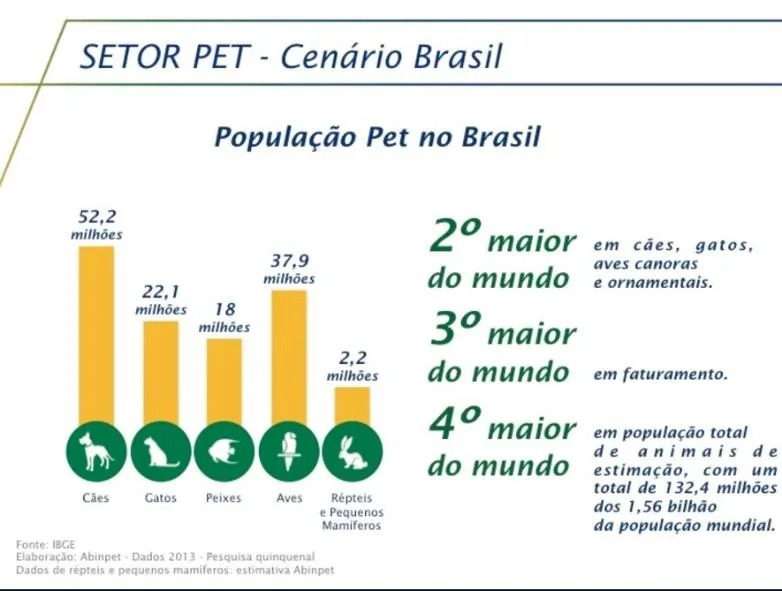
\includegraphics[scale=0.55]{/home/grmunhoz/Documents/Munhoz/University/Pictures/WhatsApp Image 2022-03-12 at 21.10.19.jpeg} 
\label{figmercado}
\legend{Fonte: \cite{abinpet}}
\end{center}
\end{figure}

O mercado pet, de acordo com a ABcomm (Associação Brasileira de Comércio Econômico), foi o detentor do 11º maior ticket médio em vendas online e movimentou cerca de 2 bilhões de reais em 2020 \cite{abcomm}. E a tendência é de que essas vendas apenas cresçam durante os próximos anos, já que o número de cães e gatos, no Brasil, pode crescer até 26$\%$ nos próximos anos. \cite{fgv}

Segundo pesquisas da COMAC (Comissão de Animais de Companhia) de 2019 e 2020, doenças renais foram uma das mais frequentes entre os animais de estimação, sendo a que mais aparece em gatos. Além disso, essas pesquisas também mostraram que a relação dos tutores com seus animais de estimação é muito forte, normalmente considerando os animais como seus filhos ou membros da família. \cite{comac}

\begin{figure}[H]
\centering
\caption{Doenças mais comuns}
\subfloat[Em cães]{
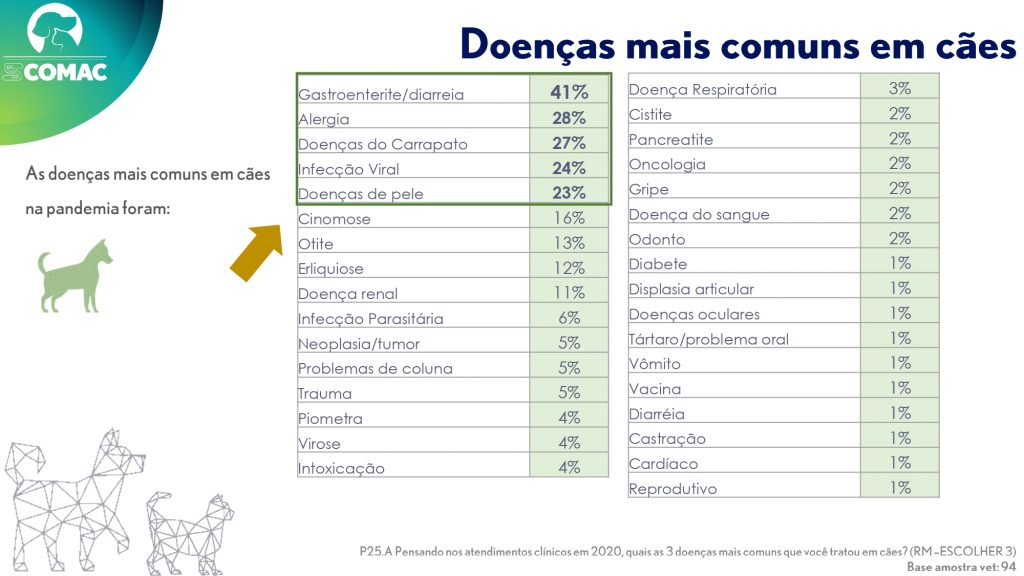
\includegraphics[scale=0.55]{../../Pictures/Apresentacao-Radar-2021-Coletiva-de-Imprensa-31.pdf_1-1024x576.jpg} 
\label{figdog}
}
\quad %espaco separador
\subfloat[Em gatos]{
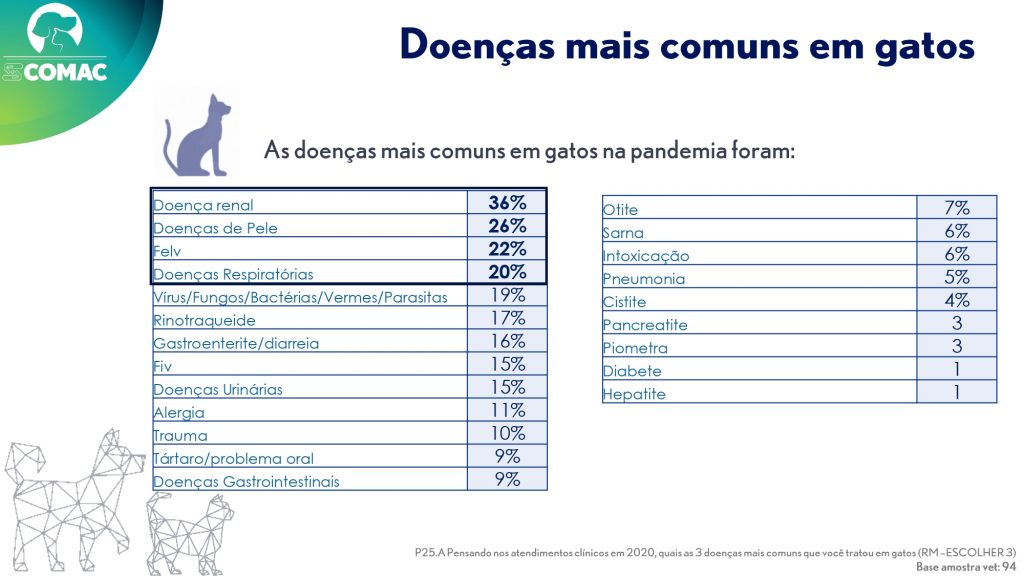
\includegraphics[scale=0.55]{../../Pictures/Apresentacao-Radar-2021-Coletiva-de-Imprensa-32.pdf_1-1024x576.jpg} 
\label{figcat}
}
\label{figdoenca}
\legend{Fonte: \cite{comac}}
\end{figure}

Outra informação importante é o gasto médio por mês que é de R\$224,60 para tutores de cães e R\$167,50 para tutores de gatos, e em relação ao gasto com acessórios por mês esse valor fica entre R\$30 e R\$40. \cite{comac}

\begin{figure}[H]
\centering
\caption{Gasto mensal com animais de estimação}
\subfloat[Média]{
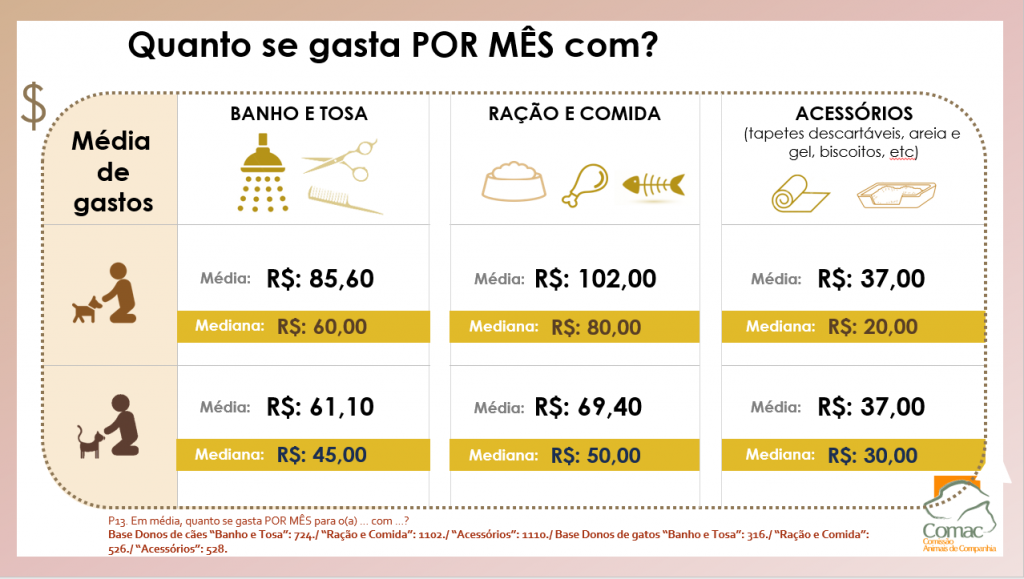
\includegraphics[scale=0.55]{/home/grmunhoz/Documents/Munhoz/University/Pictures/Radar-202029-1024x579.png} 
\label{figdog2}
}
\quad %espaco separador
\subfloat[Por classe social]{
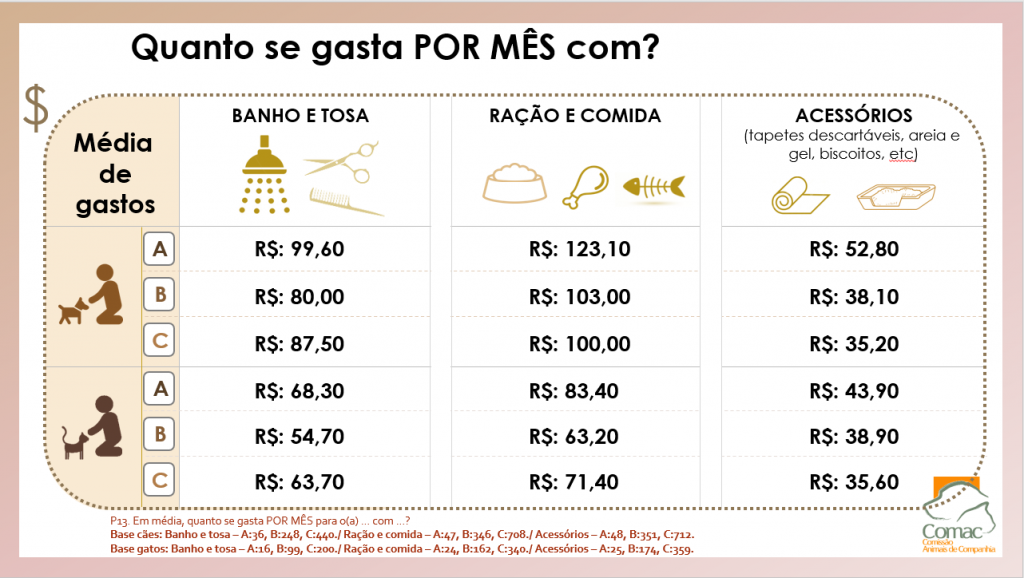
\includegraphics[scale=0.55]{/home/grmunhoz/Documents/Munhoz/University/Pictures/Radar-202030-1024x578.png} 
\label{figcat2}
}
\label{figcusto}
\legend{Fonte: \cite{comac}}
\end{figure}

A tendência de crescimento do mercado de produtos ecológicos é confirmada em diversas pesquisas, esse mercado está em expansão e nas próximas décadas vai acabar transformando o padrão de consumo mundial. Só no Brasil, entre 2019 e 2020, foram contabilizados 1,4 milhão de consumidores de produtos sustentáveis, número que cresce ano após ano. \cite{noticia}

No entanto, mesmo sendo tendência mundial, o mercado sustentável anda a passos lentos, pois o custo de matérias-primas e maquinários ainda é muito alto. “Os preços de materiais mais sustentáveis são bem mais altos. Temos que repassar isso para o produto final e, às vezes, ficamos em dúvida se o consumidor vai aceitar” afirma a empresária Ana Carolina C. C. Targa, fundadora da Barauma, empresa de calçados e acessórios veganos. \cite{folha}



\section{Revisar o PEN}

\subsection*{Compilar as informações obtidas sobre novas tendências e necessidades dos clientes}

De acordo com as informações compiladas sobre as novas tecnologias e novas tendências de mercado, haverá uma grande procura por produtos sustentáveis no futuro, o que vai ao encontro do portfólio da empresa. Segundo os dados, o mercado pet irá se desenvolver muito, já que a tendência é que aumente o número de animais de estimação em torno de 25$\%$ no Brasil até 2030 e os dados também mostram uma preocupação maior com os animais, ou seja, maiores gastos para com a saúde e alimentação dos animais. 


\subsection*{Avaliar se as metas atuais do PEN estão sendo cumpridas no prazo}

As metas do planejamento estratégico se encontram dentro do prazo e a empresa está conseguindo atingir todos os objetivos propostos.


\subsection*{Verificar se alguma nova tendência ou necessidade de mercado pode influenciar no cumprimento de alguma meta existente}

A única tendência que pode influenciar negativamente nos objetivos da empresa é que muitas outras companhias entrem no setor de sustentabilidade para desenvolvimento de materiais alternativos e sustentáveis.


\subsection*{Avaliar se existem novas oportunidades e/ou desafios para a empresa}

Um desafio para a empresa é o investimento muito alto de pesquisa e desenvolvimento para projetos de desenvolvimento de novos materiais. Enquanto, uma oportunidade é aproveitar o know-how já existente do mercado pet e produzir inovações nesse setor já que a tendência desse mercado é apenas crescer durante os próximos anos. 

\subsection*{Dimensionar, se necessário, novas metas e/ou prazos}

A meta de “se tornar uma referência nacional, em 10 anos, no ramo de desenvolvimento de produtos com materiais alternativos e ecológicos” deve ser adaptada para “se tornar referência nacional, em 10 anos, no desenvolvimento de produtos inovadores para animais de estimação”. Levando sempre como valor a sustentabilidade, porém não como prioridade.

\subsection*{Divulgar a atualização da revisão do PEN}

A empresa Okily atualizou a visão da empresa e vai focar mais no desenvolvimento de produtos inovadores para o mercado pet, ao invés do desenvolvimento de produtos em geral focados em materiais alternativos. A sustentabilidade ainda é um valor importante para a empresa, porém a prioridade da Okily mudou para o desenvolvimento de produtos inovadores exclusivos para o setor de animais de estimação.

\section{Analisar o portfólio de produtos da empresa}

A Okily possui 3 projetos em seu portfólio que deseja realizar, dois deles são
projetos que envolvem o desenvolvimento de novos materiais e o outro de um novo produto
para o mercado pet. O primeiro projeto é o desenvolvimento de um biopolímero composto
de casca de cacau, o segundo é o desenvolvimento de um papel solúvel que se torna uma
bebida em contato com água e o último é o desenvolvimento de um bebedouro com filtro
para cães e gatos feito com materiais ecológicos.

Além desses projetos a Okily já possui em seu portfólio outros produtos de materiais reciclados no mercado pet e em outros setores. Contudo, ainda não possui nenhum material alternativo criado pela empresa. 

\section{Propor mudanças no portfólio de produtos}

De acordo com as pesquisas realizadas e toda a informação coletada acerca do mercado e as tendências tecnológicas, é possível verificar que o mercado pet ainda está em grande expansão. Além disso, é fácil afirmar que a comercialização e desenvolvimento de produtos sustentáveis é dificultada pelo custo muitas vezes da matéria prima e por vezes maquinários específicos.

A Okily, no entanto, mesmo trabalhando com materiais recicláveis, não sofre com esse alto custo de matéria prima por apenas se utilizar de plásticos recicláveis já prontos para molde. Em sua gama de projetos, a empresa possui alguns relacionados com o desenvolvimento de materiais alternativos próprios. Contudo, o custo da pesquisa e do desenvolvimento somado com o provável investimento em maquinário faz com que esses projetos sejam inviáveis no presente momento.

Dessa forma, resta apenas um projeto para a empresa investir. O projeto do filtro de água para cães e gatos, diferente dos projetos de desenvolvimento de materiais faz muito sentido ser incorporado no portfólio, já que segundo as pesquisas o mercado ainda está em crescimento, a Okily possui já know-how de como funciona o setor por produzir mais produtos para pets e ainda é alinhado com o plano estratégico de negócios por possuir a vertente ambiental ao utilizar material reciclável.

Além disso, a empresa possui foco em inovação e tem como valor impactar a sociedade, então o desenvolvimento de um filtro para animais domésticos de baixo custo, com o máximo de componentes sustentáveis conseguirá ter um impacto muito forte na sociedade caso seja simples, fácil de utilizar e barato.

Ademais, outra mudança que ocorrerá no portfólio será a descontinuação de alguns produtos que não são do mercado pet. Esses produtos terão seus últimos lotes produzidos nos próximos meses. A matéria-prima e o maquinário serão utilizados na fabricação dos produtos com maior valor agregado do portfólio da empresa que é do setor de pet. 


\section{Verificar a viabilidade do portfólio de produtos}

O portfólio da Okily sempre é revisto em cada revisão do PEN para visualizar se todos os produtos que são produzidos fazem sentido em relação ao planejamento estratégico da empresa e se estão gerando receita.

Para analisar essa viabilidade a companhia, além de analisar os gastos e ganhos de cada produto, também mapeia em uma Matriz BCG quais produtos são mais importantes para a empresa e quais devem sofrer algum tipo de alteração ou se devem ser descontinuados.

A empresa atualmente possui diversos produtos no setor de animais de estimação e alguns em outros setores, então como a empresa se decidiu por focar seus esforços no setor pet os produtos não serão comparados por Matriz BCG já que a empresa conseguindo criar uma marca mais forte no mercado pet, vários produtos mesmo que menos rentáveis podem conquistar um maior market share e ultrapassar outros produtos que são de outros setores.

Assim, a Okily entende que todos os produtos do mercado pet se tornam viáveis independente de sua rentabilidade atual e que os produtos de outro setor acabam se tornando menos viáveis, pois a empresa não está mais interessada em investir nesses produtos nos próximos anos.


\section{Decidir o início do planejamento de um dos produtos do portfólio}

O produto que será desenvolvido é o filtro de água para cães e gatos, para realização do desenvolvimento desse projeto é necessário entender o mercado e a tecnologia que estará envolvida no processo. Ademais, é de grande importância analisar a viabilidade do projeto durante todo o projeto e realizar todas as fases do projeto de desenvolvimento, para que todas as características sejam de acordo com as necessidades reais do consumidor e para que o projeto consiga manter os riscos baixos.

O planejamento vai englobar a listagem dos interessados, definição de escopo do projeto e do produto, definição das atividades, o cronograma, dimensionamento de riscos e orçamento, análise de viabilidade e definição de indicadores de desempenho. Seu início começa em dias a partir da revisão do PEN e confirmação do projeto de desenvolvimento desse produto pelo departamento de P$\&$D.

\newpage
\chapter{Planejamento do Projeto}
%\pagestyle{fancy}

O planejamento do projeto será realizado no pré desenvolvimento do Processo de Desenvolvimento do Produto. Tal etapa tem como principal objetivo final a lista de projetos a serem desenvolvidos a partir da estratégia competitiva, com foco nos projetos segundo a estratégia a curto, médio e longo prazo. O filtro para cães e gatos deve ser seguido de perto por um projeto, que vai definir os interessados no projeto, definir, revisar e adaptar o escopo e a realização do levantamento de riscos e incertezas do processo de desenvolvimento.

\section{Definir interessados do projeto}

Para essa etapa, foram definidas responsabilidades de cada pessoa envolvida no projeto, a fim de detalhar o nível de dedicação e responsabilidades das pessoas envolvidas durante o processo. Para definição, utilizaremos essa legenda para responsabilidade e dedicação:

\begin{itemize}
\item \textbf{Responsabilidades:}
\subitem $\cdot$ E: Responsabilidades pela execução;
\subitem $\cdot$ A: Autoridade para aprovar;
\subitem $\cdot$ C: Precisa ser consultado;
\subitem $\cdot$ Precisa ser informado
\item \textbf{Dedicação:}
\subitem $\cdot$ I: tempo integral
\subitem $\cdot$ P(X) - Tempo parcial com X horas;
\end{itemize}

\begin{figure}[H]
\begin{center}
\caption{Responsabilidades dos interessados}
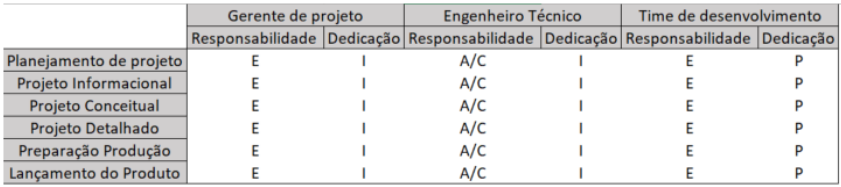
\includegraphics[scale=0.7]{/home/grmunhoz/Documents/Munhoz/University/Pictures/ScreenShot03.13.png} 
\legend{Fonte: Autoria Própria}
\end{center}
\end{figure}

\section{Definir escopo do produto}

O escopo do produto deve ser definido com todas as partes envolvidas no projeto, em reuniões direcionadas pelo gerente de projeto, onde esse deve estudar a Minuto do Projeto, podendo assim definir as diretrizes que o produto deverá atender. Deve ser definido também pontos como o que é o produto e quais suas finalidades no mercado. 

{\fontsize{10}{15}\selectfont
\begin{center}
\begin{longtable}[c]{|
>{\columncolor[HTML]{9FC5E8}}l l|}
\caption{Escopo do Produto}
\label{tableproduto3}\\
\hline
\multicolumn{2}{|c|}{\cellcolor[HTML]{9FC5E8}\textbf{Escopo do Produto}}                                                      \\ \hline
\endhead
%
\multicolumn{1}{|l|}{\cellcolor[HTML]{9FC5E8}O que é?}                & Filtro para cães e gatos;                             \\ \hline
\multicolumn{1}{|l|}{\cellcolor[HTML]{9FC5E8}Vida útil.}              & Vida útil do filtro: 2 meses;                         \\ \hline
\multicolumn{1}{|l|}{\cellcolor[HTML]{9FC5E8}Funcionalidade.} &
  \begin{tabular}[c]{@{}l@{}}Através de materiais ecológicos, proporcionar para o mercado pet, \\ um filtro que diminua as impurezas da água consumida por cães e gatos;\end{tabular} \\ \hline
\multicolumn{1}{|l|}{\cellcolor[HTML]{9FC5E8}Embalagem (Un).}         & Embalagem plástica com preço de custo de 22 centavos; \\ \hline
\multicolumn{1}{|l|}{\cellcolor[HTML]{9FC5E8}Materiais.} &
  \begin{tabular}[c]{@{}l@{}}Embalagem: plástico;\\ Refil: carvão ativado, Quartzo, Dolomita e Alumina;\\ Outros: haste de metal;\end{tabular} \\ \hline
\multicolumn{1}{|l|}{\cellcolor[HTML]{9FC5E8}Especialista envolvido.} & Engenheiro técnico;                                   \\ \hline
\multicolumn{1}{|l|}{\cellcolor[HTML]{9FC5E8}Peso filtro.}            & 0.329 kg;                                             \\ \hline
\end{longtable}
\centering \footnotesize{Fonte: Autoria Própria}
\end{center}
}


\section{Definir escopo do projeto}

Após a definição do escopo do produto, devemos estabelecer como esse produto será obtido, ou seja, o conjunto de atividades que serão executadas para construir e entregar o produto para o mercado consumidor.

{\small
\begin{center}
\begin{longtable}[c]{|ll|}
\caption{Escopo do Projeto}
\label{tableproduto3}\\
\hline
\multicolumn{2}{|c|}{\cellcolor[HTML]{9FC5E8}\textbf{Gerenciamento de Escopo do Projeto}} \\ \hline
\endhead
%
\multicolumn{2}{|l|}{\cellcolor[HTML]{9FC5E8}Justificativa do projeto:} \\ \hline
\multicolumn{2}{|l|}{\begin{tabular}[c]{@{}l@{}}Este projeto tem como justificativa a gerir o desenvolvimento do produto Filtro para Pet. \\ Com atividades que tornem o produto competitivo no mercado, tendo como público alvo \\ donos de cães e gatos, buscando alinhar a equipe que trabalhará com o projeto, elaborar \\ cronogramas de cada etapa, definir as atividades do desenvolvimento e analisar o ciclo \\ de vida do produto, alinhando também o processo de desenvolvimento com a estratégia \\ competitiva da empresa.\end{tabular}} \\ \hline
\multicolumn{2}{|l|}{\cellcolor[HTML]{CFE2F3}Escopo do produto:} \\ \hline
\multicolumn{2}{|l|}{\begin{tabular}[c]{@{}l@{}}Suporte de plástico adaptável a diferentes tamanhos de recipientes;\\ Filtro à base de carvão mineral;\\ Filtro a base de materiais ecológicos;\end{tabular}} \\ \hline
\multicolumn{2}{|l|}{\cellcolor[HTML]{9FC5E8}Cronograma do Projeto.} \\ \hline
\multicolumn{2}{|l|}{O projeto terá duração total de 102 dias.} \\ \hline
\multicolumn{2}{|l|}{\cellcolor[HTML]{CFE2F3}Restrições identificadas.} \\ \hline
\multicolumn{2}{|l|}{\begin{tabular}[c]{@{}l@{}}Ser adaptável a diferentes raças de cães e gatos;\\ Desenvolvimento de um produto sustentável;\\ Ter um custo acessível para atingir diversos públicos;\end{tabular}} \\ \hline
\multicolumn{2}{|l|}{\cellcolor[HTML]{9FC5E8}Equipe envolvida no desenvolvimento:} \\ \hline
\multicolumn{2}{|l|}{\begin{tabular}[c]{@{}l@{}}O projeto será gerido pelo Gerente de Projetos, que terá um suporte técnico do Engenheiro \\ especialista, responsável pelas aprovações e especificações técnicas e uma equipe \\ multidisciplinar denominada Time de Desenvolvimento, responsável pelo desenvolvimento \\ do produto em questão.\end{tabular}} \\ \hline
\end{longtable}
\centering \footnotesize{Fonte: Autoria Própria}
\end{center}
}


%\section{Detalhar o escopo do projeto}

\section{Adaptar o modelo de referência}

O modelo de referência é dividido em Pré, Desenvolvimento e Pós. O principal objetivo é envolver as atividades de definição de projeto de desenvolvimento a partir da estratégia competitiva da empresa e realizar o acompanhamento do produto até sua descontinuidade no mercado. O Filtro para cães e gatos trata-se de um novo produto, mas em um segmento conhecido pela empresa, por conta de outros produtos atuantes na mesma área. Apesar de apresentar uma inovação no quesito ecológico, o projeto não apresenta uma complexidade muito alta. Portanto, podemos unificar duas fases do modelo de referência de Rozenfeld do Projeto Informacional e Projeto Conceitual.

\section{Preparar cronograma e atividades}

Após definir e sequenciar as atividades, é necessário definir o tempo de início e fim do projeto, ou seja, definir um cronograma das atividades.

%{\small
\begin{center}
\begin{longtable}[c]{|l|l|l|l|}
\caption{Cronograma de atividades}
\label{tableproduto3}\\
\hline
\rowcolor[HTML]{9FC5E8} 
\textbf{Fase}                     & \textbf{Duração} & \textbf{Início} & \textbf{Término} \\ \hline
\endhead
%
Planejamento do Produto           & 45               & 04/04/2022      & 03/06/2022       \\ \hline
Gerenciamento de projeto          & 2                & 06/06/2022      & 07/06/2022       \\ \hline
Escopo                            & 2                & 08/06/2022      & 09/06/2022       \\ \hline
Definição de requisitos           & 1                & 10/06/2022      & 10/06/2022       \\ \hline
Definir objetivo do produto       & 2                & 13/06/2022      & 14/062022        \\ \hline
Projeto Detalhado                 & 5                & 15/06/2022      & 21/06/2022       \\ \hline
Elaborar modelo                   & 5                & 22/06/2022      & 28/06/2022       \\ \hline
Detalhar características técnicas & 4                & 29/06/2022      & 01/07/2022       \\ \hline
Aprimorar design                  & 2                & 04/07/2022      & 05/07/2022       \\ \hline
Obter matéria prima               & 10               & 06/07/2022      & 19/07/2022       \\ \hline
Aquisição de máquinas             & 20               & 22/07/2022      & 12/08/2022       \\ \hline
Analisar viabilidade econômica    & 2                & 15/08/2022      & 16/08/2022       \\ \hline
Analisar riscos                   & 2                & 17/0/2022       & 18/08/2022       \\ \hline
Produção de protótipos            & 10               & 19/08/2022      & 01/09/2022       \\ \hline
\end{longtable}
\centering \footnotesize{Fonte: Autoria Própria}
\end{center}
%}

\section{Avaliar riscos}

Para avaliação de riscos e incertezas que podem acompanhar o desenvolvimento do produto e projeto, será utilizado a metodologia da análise SWOT que consiste em um diagrama que é dividido em quatro quadrantes com o objetivo de avaliar características do Ambiente Interno - forças e fraquezas -  e características do Ambiente Externos - ameaças e oportunidades.

\begin{itemize}
\item \textbf{Forças}
\subitem $\cdot$ Sustentabilidade;
\subitem $\cdot$ Preocupação com o bem estar dos pets;
\subitem $\cdot$ Aumento do número de Lares com pets;,
\subitem $\cdot$ Inovação;
\subitem $\cdot$ Preocupação ecológica;
\item \textbf{Fraquezas}
\subitem $\cdot$ Material complexo;
\subitem $\cdot$ Custo de produto;
\item \textbf{Oportunidades}
\subitem $\cdot$ Aumento do número de Lares com pets;
\subitem $\cdot$ Crescimento do mercado de produtos ecológicos;
\item \textbf{Ameaças}
\subitem $\cdot$ Importância do produto no mercado externo;
\end{itemize}

\section{Preparar orçamento do projeto}

Para a realização e compilação do orçamento do projeto é necessário algumas informações anteriores, são essas:

\begin{itemize}
\item \textbf{Custo unitário do produto:} O custo unitário do produto referenciado é de R\$11,46 sendo considerados nessa conta todos os custos diretos.

\begin{figure}[H]
\begin{center}
\caption{Cálculo do custo unitário do produto}
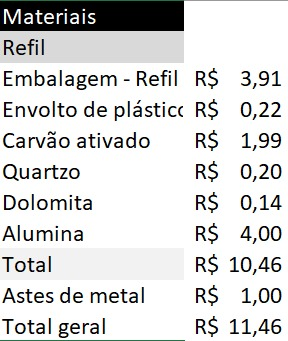
\includegraphics[scale=0.5]{/home/grmunhoz/Documents/Munhoz/University/Pictures/download (3).jpeg} 
\legend{Fonte: Autoria Própria}
\end{center}
\end{figure}

\item \textbf{Recurso humano}
	\subitem $\cdot$ Para o desenvolvimento do projeto são necessárias 4 pessoas, sendo 4 integrantes do grupo. Considerando que o custo hora médio no Brasil está por volta de R\$8,50 se faz possível ter um parâmetro geral do recurso humano utilizado:
	
\begin{figure}[H]
\begin{center}
\caption{Recurso humano projetado}
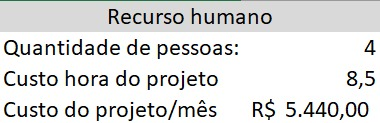
\includegraphics[scale=0.5]{/home/grmunhoz/Documents/Munhoz/University/Pictures/download (1).jpeg} 
\legend{Fonte: Autoria Própria}
\end{center}
\end{figure}	
	
\item \textbf{Custos com maquinário}
	\subitem $\cdot$ Esteira para a produção de refil
	
\begin{figure}[H]
\begin{center}
\caption{Esteira}
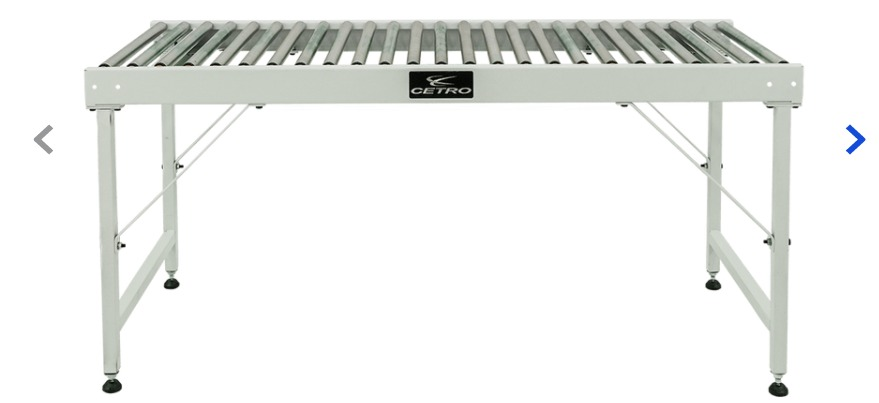
\includegraphics[scale=0.4]{/home/grmunhoz/Documents/Munhoz/University/Pictures/download.jpeg} 
\legend{Fonte: Autoria Própria}
\end{center}
\end{figure}		
	
	\subitem $\cdot$ Injetoras para a injeção de plástico e formação da carcaça do refil
	
\begin{figure}[H]
\begin{center}
\caption{Injetoras}
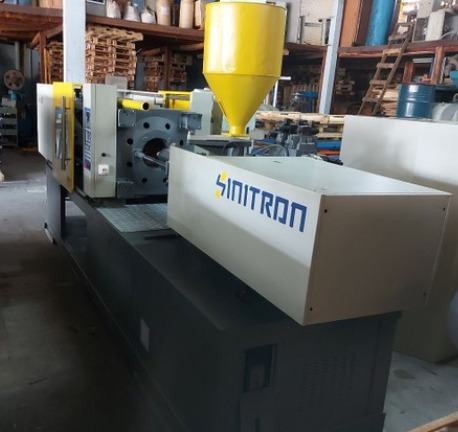
\includegraphics[scale=0.4]{/home/grmunhoz/Documents/Munhoz/University/Pictures/download (2).jpeg} 
\legend{Fonte: Autoria Própria}
\end{center}
\end{figure}		
	
	\subitem $\cdot$ Custo do maquinário

\begin{figure}[H]
\begin{center}
\caption{Custo do maquinário}
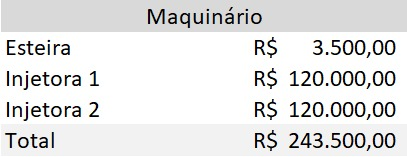
\includegraphics[scale=0.5]{/home/grmunhoz/Documents/Munhoz/University/Pictures/download (4).jpeg} 
\legend{Fonte: Autoria Própria}
\end{center}
\end{figure}	

\end{itemize}

Portanto, o orçamento geral do projeto é o seguinte:

\begin{figure}[H]
\begin{center}
\caption{Orçamento geral do projeto}
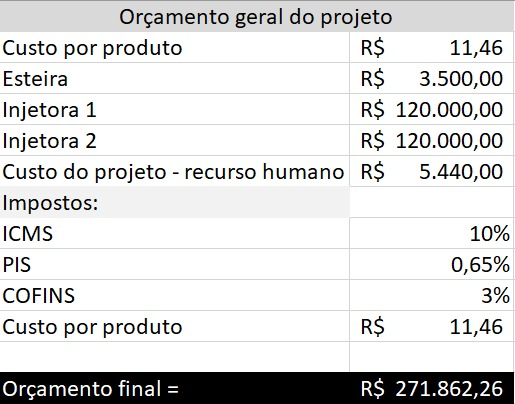
\includegraphics[scale=0.5]{/home/grmunhoz/Documents/Munhoz/University/Pictures/WhatsApp Image 2022-03-13 at 16.43.44.jpeg} 
\legend{Fonte: Autoria Própria}
\end{center}
\end{figure}	

\section{Analisar a viabilidade econômica do projeto}

A análise da viabilidade econômica permite a avaliação do projeto como um todo, no sentido de este ser ou não viável principalmente no quesito financeiro.

\begin{itemize}
\item \textbf{Precificação:}

\begin{figure}[H]
\begin{center}
\caption{Precificação}
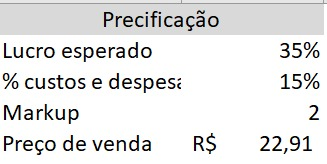
\includegraphics[scale=0.5]{/home/grmunhoz/Documents/Munhoz/University/Pictures/download (6).jpeg} 
\legend{Fonte: Autoria Própria}
\end{center}
\end{figure}	

\item \textbf{VPL:}
\subitem O valor presente líquido é uma equação econômico financeira capaz de determinar o valor presente de pagamentos futuros descontados a uma taxa pré-determinada e diferente dependendo de cada tipo de empreendimento, negócio o pagamento, retirando o custo inicial investido;
\subitem Para o produto analisado até o momento, considerando todo o investimento inicial e o valor futuro de vendas, o VPL resulta na seguinte análise:

\begin{figure}[H]
\begin{center}
\caption{VPL}
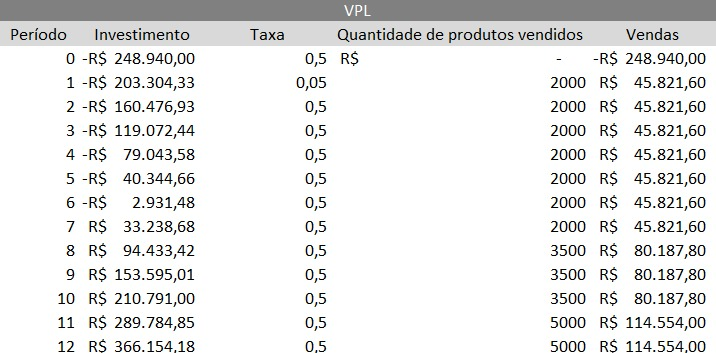
\includegraphics[scale=0.5]{/home/grmunhoz/Documents/Munhoz/University/Pictures/VPL.jpeg} 
\legend{Fonte: Autoria Própria}
\end{center}
\end{figure}	

\begin{figure}[H]
\begin{center}
\caption{Gráfico do VPL}
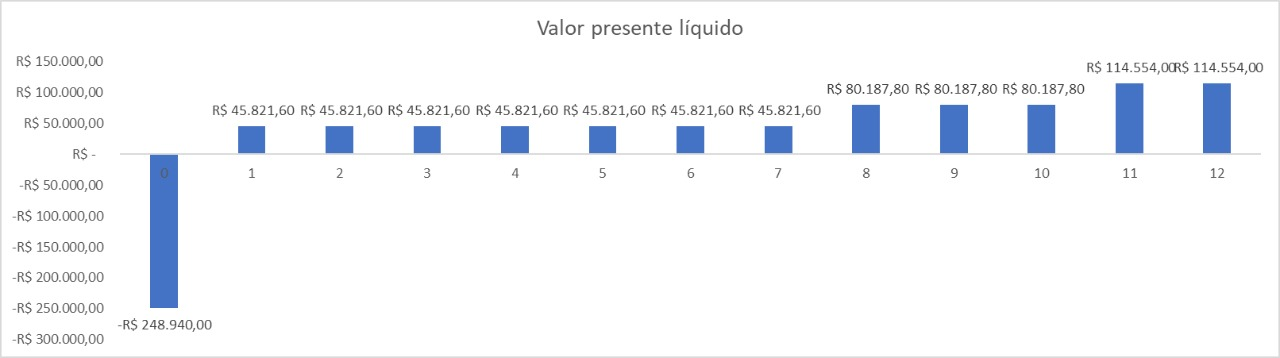
\includegraphics[scale=0.35]{/home/grmunhoz/Documents/Munhoz/University/Pictures/vplgrafico.jpeg} 
\legend{Fonte: Autoria Própria}
\end{center}
\end{figure}	

\item \textbf{TIR:}

\begin{figure}[H]
\begin{center}
\caption{TIR}
\includegraphics[scale=0.43]{/home/grmunhoz/Documents/Munhoz/University/Pictures/tir.jpeg} 
\legend{Fonte: Autoria Própria}
\end{center}
\end{figure}	

\item \textbf{Payback:}

\begin{figure}[H]
\begin{center}
\caption{Payback}
\includegraphics[scale=0.43]{/home/grmunhoz/Documents/Munhoz/University/Pictures/payback.jpeg} 
\legend{Fonte: Autoria Própria}
\end{center}
\end{figure}	

\end{itemize}


\section{Definir indicadores de desempenho}

Os indicadores de desempenho tem como intuito principal acompanhar de forma simples e direta o andamento do projeto, bem como se as restrições do projeto estão sendo respeitadas, como por exemplo a alocação de todos os recursos. Os seguintes indicadores foram pré-selecionados para o bom andamento do projeto e o atingimento dos objetivos estratégicos, táticos e operacionais.

\begin{itemize}
\item \textbf{Custo total do projeto:} Para ter o controle da utilização dos recursos em geral para o desenvolvimento do projeto;
	\subitem $\cdot$ Somatório de todos os custos do projeto até aquele momento.
\item \textbf{Tempo por atividade:} Com esse indicador é possível analisar o desempenho e a produtividade por pessoa e por atividade;
	\subitem $\cdot$ Somatória do tempo demandado por atividade.
\item \textbf{Índice de atividades atingidas vs planejado:} Indicará o percentual de atividades concluídas, gerando um relatório e análises de produtividade e desempenho, além de prever o prazo de término do projeto;
	\subitem $\cdot$ (Quantidade de atividades finalizadas/Quantidade de atividades do projeto) * 100.
\item \textbf{Recursos financeiros utilizados vs planejado (Assertividade do planejamento financeiro):}
	\subitem $\cdot$ (Recursos utilizados / recursos para o projeto)*100.
		\subsubitem $\cdot$ Caso for maior que 100$\%$ o projeto ultrapassou o valor projetado;
\end{itemize}

\section{Definir plano de comunicação}

A comunicação da equipe acontecerá conforme a necessidade, sendo possível utilizar de múltiplos canais, tais como por meio do whatsapp, Email e Trello, sendo que cada um desses canais serão utilizados para um objetivo distinto:

\begin{itemize}
\item \textbf{Whatsapp:}
	\subitem $\cdot$ Quando há urgência na atividade a ser realizada ou no alinhamento requerido no momento.
\item \textbf{Email:} 	
	\subitem $\cdot$ Marcar reuniões de cunho mais formal;
	\subitem $\cdot$ Comunicados com um grau de urgência menor.
\item \textbf{Trello:}
	\subitem $\cdot$ Com objetivo de delegação de atividades de forma mais flexível e direta;
	\subitem $\cdot$ Voltado para cobranças indiretas às atividades atrasadas, mesmo não iniciadas ou até mesmo novas tarefas.
\end{itemize}

\section{Planejar e preparar aquisições}

O planejamento das aquisições deve ser muito bem feita e pensada, uma vez que esse investimento corresponde a maior parte dos recursos disponíveis, já que caso tal planejamento esteja errado de alguma forma, todo o projeto pode ser prejudicado.

Para a realização do planejamento de aquisições, será dividido em algumas etapas:

\begin{itemize}
\item \textbf{Matéria prima necessária para produção de um produto:}
	\subitem $\cdot$ Estoque de matéria prima, necessidade mínima de matéria prima para a produção de pelo menos 2000 produtos.
\item \textbf{Análise e comparação dos fornecedores:}
	\subitem $\cdot$ Mapeamento dos fornecedores;
	\subitem $\cdot$ Cotação com os mesmos fornecedores;
	\subitem $\cdot$ Comparação entre melhor tempo/qualidade/custo na entrega.
\item \textbf{Necessidade de aquisições:}
	\subitem $\cdot$ 2 Injetoras;
	\subitem $\cdot$ Esteira - produção do refil.
\end{itemize}
\section{Preparar plano de projeto}

%\begin{landscape}
\begin{figure}[H]
\begin{center}
\caption{Project Charter}
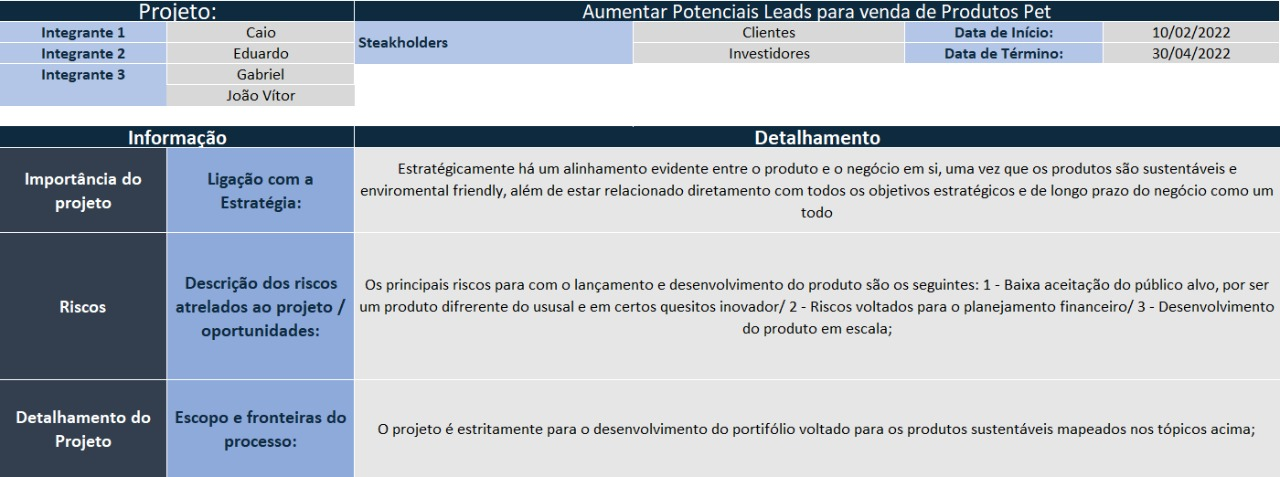
\includegraphics[scale=0.36]{/home/grmunhoz/Documents/Munhoz/University/Pictures/3.14 - Project Charter.jpeg} 
\label{figprojeto}
\legend{Fonte: Autoria Própria}
\end{center}
\end{figure}
%\end{landscape}

\newpage
\chapter{Projeto Informacional}
%\pagestyle{fancy}

Conforme Rozenfeld et al. (2017), esta fase caracteriza-se pelas atividades da equipe de projetos em relacionar a busca, criação, representação e seleção de soluções para o problema do projeto. Dessa forma nesta etapa iremos levar em conta a percepção do público alvo para definir os requisitos do cliente e relacionar esses requisitos com os requisitos do produto. \cite{rozenfeld}

A partir das análises podemos identificar os pontos de maior importância na visão do cliente, ou seja, que agregam maior valor ao produto final e fazer uma correlação desses pontos com as especificações do nosso produto. Assim definindo metas para essas especificações e melhorando elas, poderemos refletir no produto as qualidades desejadas pelo cliente.

Para fazer isso utilizamos nessa etapa o conceito da matriz QFD.


\section{Revisar e atualizar o escopo do produto}

O escopo do produto, anteriormente definido, especifica características relacionas a apresentação do produto, vida útil, funcionalidade, tipo de embalagem, materiais, responsáveis e peso. Como mostra na figura abaixo.

{\fontsize{10}{15}\selectfont
\begin{center}
\begin{longtable}[c]{|
>{\columncolor[HTML]{9FC5E8}}l l|}
\caption{Escopo do Produto}
\label{tableproduto3}\\
\hline
\multicolumn{2}{|c|}{\cellcolor[HTML]{9FC5E8}\textbf{Escopo do Produto}}                                                      \\ \hline
\endhead
%
\multicolumn{1}{|l|}{\cellcolor[HTML]{9FC5E8}O que é?}                & Filtro para cães e gatos;                             \\ \hline
\multicolumn{1}{|l|}{\cellcolor[HTML]{9FC5E8}Vida útil.}              & Vida útil do filtro: 2 meses;                         \\ \hline
\multicolumn{1}{|l|}{\cellcolor[HTML]{9FC5E8}Funcionalidade.} &
  \begin{tabular}[c]{@{}l@{}}Através de materiais ecológicos, proporcionar para o mercado pet, \\ um filtro que diminua as impurezas da água consumida por cães e gatos;\end{tabular} \\ \hline
\multicolumn{1}{|l|}{\cellcolor[HTML]{9FC5E8}Embalagem (Un).}         & Embalagem plástica com preço de custo de 22 centavos; \\ \hline
\multicolumn{1}{|l|}{\cellcolor[HTML]{9FC5E8}Materiais.} &
  \begin{tabular}[c]{@{}l@{}}Embalagem: plástico;\\ Refil: carvão ativado, Quartzo, Dolomita e Alumina;\\ Outros: haste de metal;\end{tabular} \\ \hline
\multicolumn{1}{|l|}{\cellcolor[HTML]{9FC5E8}Especialista envolvido.} & Engenheiro técnico;                                   \\ \hline
\multicolumn{1}{|l|}{\cellcolor[HTML]{9FC5E8}Peso filtro.}            & 0.329 kg;                                             \\ \hline
\end{longtable}
\centering \footnotesize{Fonte: Autoria Própria}
\end{center}
}

Levando em consideração uma pesquisa com público reduzido podemos identificar alguns pontos de melhoria ou de maior atenção dentro deste escopo. 

Dentro do que é o nosso produto entendemos que não só é um filtro para cães e gatos como deve ser acessível a todas as pessoas que tem pet. Tendo em vista isso identificamos que a vida útil do produto é um empecilho, pois quando comparamos nosso filtro com outros filtros de pet já existentes vemos que o nosso tem o preço muito competitivo, porém em comparação a recipientes mais simples, que não utilizam de filtro, estamos com valor bem acima. Portanto precisamos aumentar a vida útil desse produto para torna-lo mais atrativo às pessoas que ainda não utilizam nenhum tipo de filtro para pets.

Outro ponto analisado foi que a comodidade de não ter que trocar frequentemente a água do pet e não ter que se preocupar com sujeira é um ponto importante na visão dos clientes, portanto definimos que a capacidade do reservatório é uma característica importante e definimos uma meta de 2L de capacidade do reservatório.

Esses foram os principais pontos levantados, entretanto todos os itens destacados no escopo foram comparados também com produtos concorrentes no mercado e de acordo com a sua importância foi definido um índice de melhoria de acordo com a matriz QFD.


\section{Detalhar ciclo de vida do produto e definir seus clientes}

O ciclo de vida do produto na visão de mercado tem um fluxo simples que atinge praticamente todo tipo de produto, esse ciclo vai desde o seu planejamento até a fase da sua descontinuação no mercado (Figura \ref{figetapas}). Os produtos diferem pelos tempos em que atingem esses estágios e a ideia do desenvolvimento do produto é planejar de forma que esse produto se mantenha o maior tempo possível nos estágios de crescimento e maturidade.

\begin{figure}[H]
\begin{center}
\caption{Etapas do ciclo de vida com base no processo de PDP}
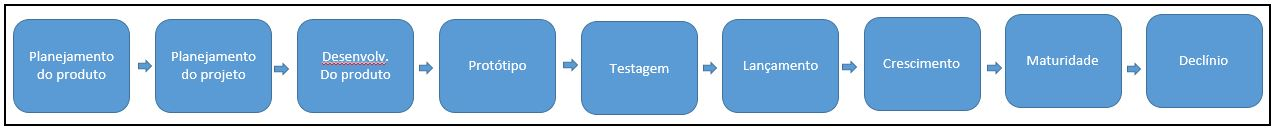
\includegraphics[scale=0.7]{/home/grmunhoz/Documents/Munhoz/University/Pictures/etapas.JPG} 
\label{figetapas}
\legend{Fonte: Autoria Própria}
\end{center}
\end{figure}

Olhando para o ciclo de vida do produto durante seu processo de produção até seu descarte planejamos um ciclo fechado, onde nada é perdido e seguindo nossos valores de sustentabilidade.

Assim o descarte do próprio produto pode tornar-se matéria-prima para a produção de novos desses mesmos produtos, gerando contribuições para o meio ambiente e ajudando a tornar o produto mais barato e acessível a todos os clientes e ajudando a melhorar a qualidade de vida dos pets.

\begin{figure}[H]
\begin{center}
\caption{Ciclo de vida com base no uso do produto}
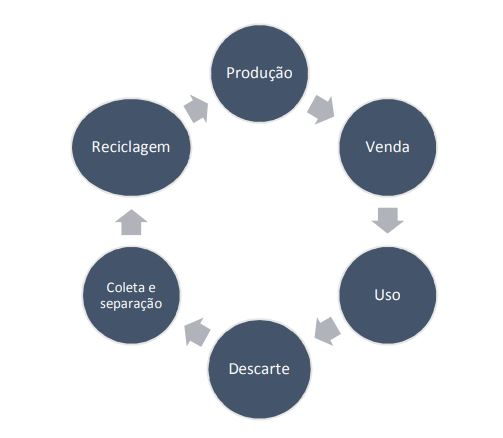
\includegraphics[scale=1]{/home/grmunhoz/Documents/Munhoz/University/Pictures/ciclo.JPG} 
\label{figciclo}
\legend{Fonte: Autoria Própria}
\end{center}
\end{figure}

Analisando a imagem anterior, que define o ciclo de vida do produto, podemos identificar os clientes das diferentes etapas do ciclo.

Na etapa de produção temos os clientes internos representados pelos setores de desenvolvimento e planejamento, que recebem a ideia e as matérias-primas e são responsáveis pela produção do item dentro das especificações meta.

Em seguida temos os clientes intermediários que podem ser representados por revendedores ou pelo cliente final que utiliza o produto. O cliente final do produto consiste em pessoas que possuem algum pet (gato ou cachorro) e preocupam-se com a qualidade de vida do animal e com sustentabilidade. Esses clientes são responsáveis pela etapa de uso até o descarte.

As etapas de coleta e separação e reciclagem podem ser realizadas pela própria empresa, no modelo em que o cliente devolve o produto ao final da sua vida e recebe benefícios para a compra de novos produtos. Tanto quanto por empresas privadas ou pela reciclagem feita pelo próprio cliente para uso do material com outra finalidade após o fim da sua vida útil como filtro.


\section{Identificar os requisitos dos clientes do produto}

Através de uma pesquisa em escala reduzida com o público alvo do produto (donos de pet com preocupação com a qualidade de vida e meio ambiente) foi possível entender alguns pontos que seriam importantes no produto pela visão do cliente.

Dessa forma os requisitos elencados após a pesquisa foram:

\begin{figure}[H]
\begin{center}
\caption{Requisitos dos clientes}
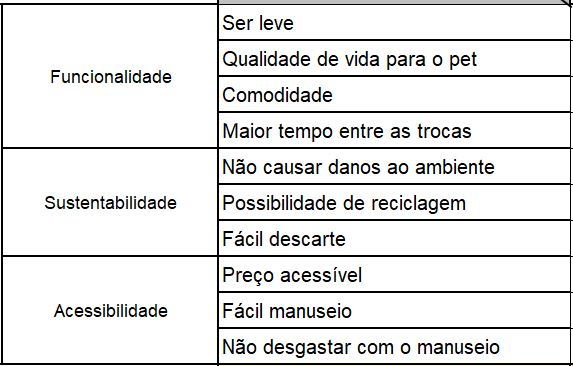
\includegraphics[scale=0.9]{/home/grmunhoz/Documents/Munhoz/University/Pictures/req. cliente.JPG} 
\legend{Fonte: Autoria Própria}
\end{center}
\end{figure}

\section{Definir os requisitos do produto}

Analisando os requisitos dos clientes e as especificações do produto, foram destacados algumas características que na visão do planejamento serão os pontos onde poderemos ter maior valor agregado ao produto.

Essas características se relacionam com os requisitos de funcionalidade, sustentabilidade e acessibilidade, mesmo que em algumas não seja tão visível pelos olhos do cliente final. São elas:

\begin{figure}[H]
\begin{center}
\caption{Requisitos do produto}
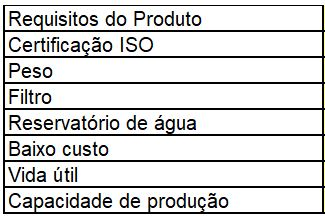
\includegraphics[scale=0.9]{/home/grmunhoz/Documents/Munhoz/University/Pictures/req. produto.JPG} 
\legend{Fonte: Autoria Própria}
\end{center}
\end{figure}


\section{Definir especificações-meta do produto}

A partir dos requisitos definidos foi utilizado a matriz QFD para fazer uma análise desses requisitos e chegar nas especificações-meta do produto. Matriz QFD (Quality Function Deployment), que significa Desdobramento da Função Qualidade, é um método que busca garantir a qualidade durante o processo de desenvolvimento de produtos e serviços.

Em primeiro lugar, esse método consiste em ouvir a voz do cliente para desenvolver produtos ou serviços por meio de diversos fatores como funções do produto, qualidade, processos, entre outros.

Como resultado tivemos o índice de melhoria no nosso produto em relação aos requisitos apresentados pelo cliente:

\begin{figure}[H]
\begin{center}
\caption{Índice de melhoria dos requisitos}
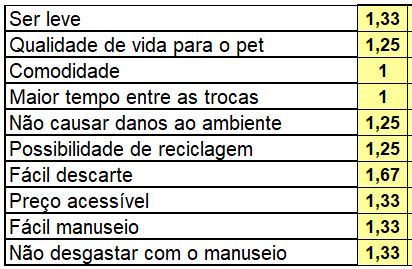
\includegraphics[scale=1]{/home/grmunhoz/Documents/Munhoz/University/Pictures/IM.JPG} 
\legend{Fonte: Autoria Própria}
\end{center}
\end{figure}

O índice de melhoria representa a oportunidade de melhoria que temos em cada requisito, levando em consideração a avaliação desse requisito no nosso produto em comparação aos concorrentes e a importância geral que o cliente enxerga nesse requisito. Podemos interpretar esse índice através da lógica:

\begin{center}
$\%$ de melhoria = (IM – 1)x100
\end{center}

Posteriormente através da análise dos requisitos dos clientes conseguimos construir uma correlação desses requisitos com os requisitos do produto e classifica-los de acordo com a importância de cada característica.

O resultado obtido para o produto foi:

\begin{figure}[H]
\begin{center}
\caption{Valor de importância}
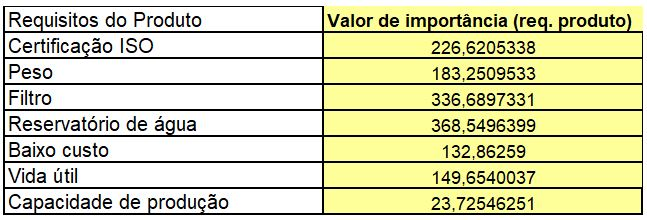
\includegraphics[scale=1]{/home/grmunhoz/Documents/Munhoz/University/Pictures/Importancia.JPG} 
\legend{Fonte: Autoria Própria}
\end{center}
\end{figure}

A importância dada para cada característica leva em conta a relação dessa característica com os requisitos do cliente, o grau de importância desses requisitos e o argumento de vendas (ou seja, o apelo que uma determinada característica apresenta para potencializar a aceitação e vendas do produto).

Pelos resultados obtidos podemos ver que as características com maior importância são: Reservatório de água, filtro e certificações ISO.

Por fim com todos os índices anteriormente definidos chegamos as especificações meta do nosso produto que ficaram de acordo com a tabela abaixo:

\begin{figure}[H]
\begin{center}
\caption{Especificações-meta do produto}
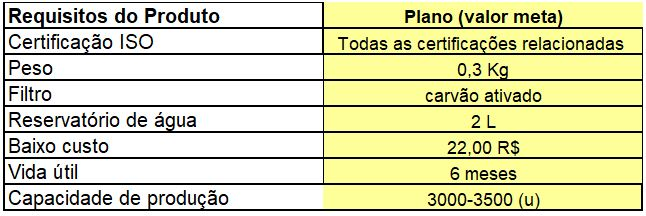
\includegraphics[scale=1]{/home/grmunhoz/Documents/Munhoz/University/Pictures/especificacoes.JPG} 
\legend{Fonte: Autoria Própria}
\end{center}
\end{figure}

\newpage
\chapter{Projeto Conceitual}
%\pagestyle{fancy}

\section{Modelar funcionalmente}

Como função global, o filtro de água para pets, tem como principal objetivo retirar as impurezas da água, tornando-a assim, própria para o consumo.

\begin{figure}[H]
\begin{center}
\caption{Funcionamento do produto de forma resumida}
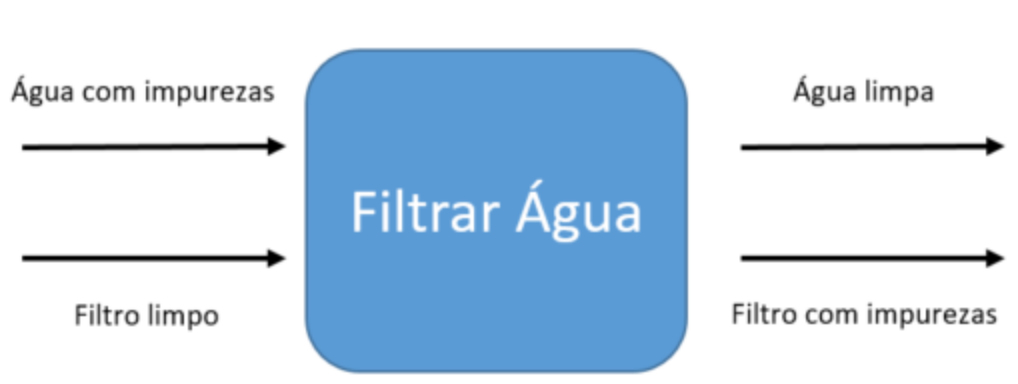
\includegraphics[scale=0.3]{/home/grmunhoz/Documents/Munhoz/University/Pictures/agua.png} 
\label{figetapas}
\legend{Fonte: Autoria Própria}
\end{center}
\end{figure}

Como entrada do nosso processo de funcionamento, temos a água contendo impurezas, e a utilização de um filtro limpo, que deve ser trocado de seis em seis meses. Como saída, temos a água limpa, própria para o consumo dos pets, e o filtro com as impurezas retiradas da água.

\begin{figure}[H]
\begin{center}
\caption{Funcionamento do produto detalhado}
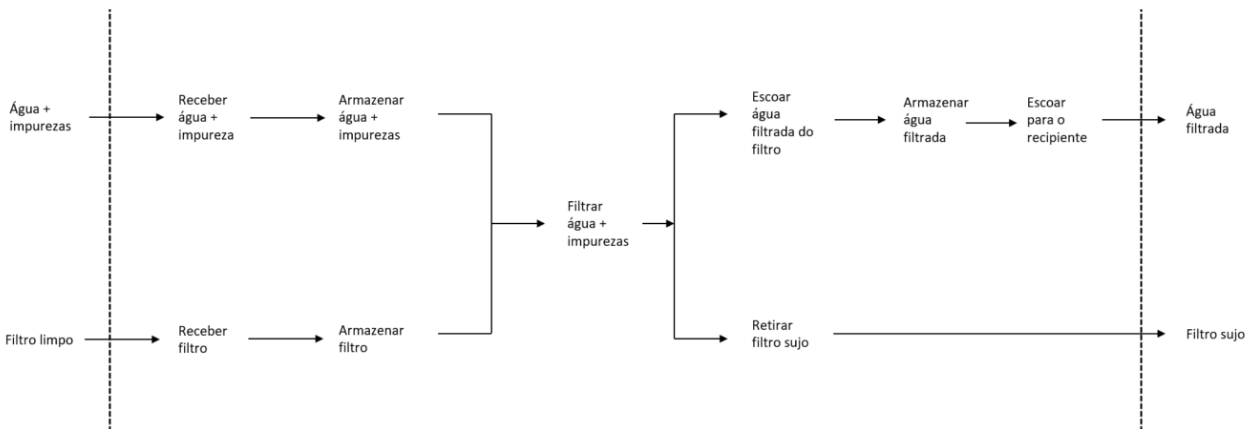
\includegraphics[scale=0.5]{/home/grmunhoz/Documents/Munhoz/University/Pictures/fluxo.png} 
\label{figetapas}
\legend{Fonte: Autoria Própria}
\end{center}
\end{figure}


\section{Desenvolver princípios de soluções para as funções}

Para o desenvolvimento dos princípios de soluções para as funções, foi utilizado o método de criatividade da matriz morfológica. A metodologia consiste no desdobramento de um problema complexo e partes mais simples, e combinando as diferentes funções, com os princípios de solução, busca a melhor combinação para o desenvolvimento do produto.


\section{Desenvolver alternativas de solução}

A metodologia foi aplicada para resolver dois principais problemas no desenvolvimento do produto. O primeiro, como seria a inserção da água no início do processo de uso. O segundo problema, como seria armazenada a água após a filtragem, ou seja, como o pet beberia a água filtrada. Com a aplicação da metodologia, chegamos em três principais alternativas para a solução do problema:

\begin{figure}[H]
\begin{center}
\caption{Alternativas de solução}
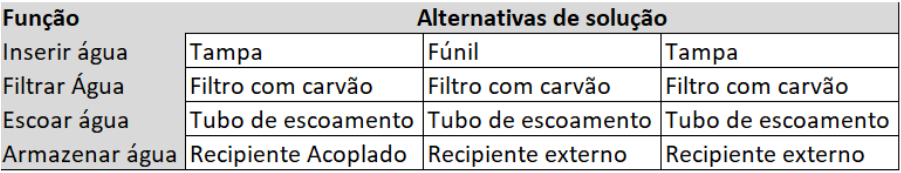
\includegraphics[scale=0.65]{/home/grmunhoz/Documents/Munhoz/University/Pictures/alternativas.png} 
\label{figetapas}
\legend{Fonte: Autoria Própria}
\end{center}
\end{figure}

\section{Definir arquitetura}

Como será especificado nos próximos tópicos, a alternativa de solução escolhida foi o produto com tampa e com o recipiente acoplado:

\begin{figure}[H]
\begin{center}
\caption{Alternativas de solução}
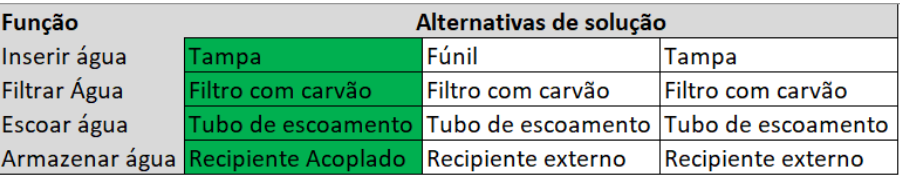
\includegraphics[scale=0.65]{/home/grmunhoz/Documents/Munhoz/University/Pictures/funcao.png} 
\label{figetapas}
\legend{Fonte: Autoria Própria}
\end{center}
\end{figure}


A escolha da tampa foi por conta da praticidade quando necessário o reabastecimento. O recipiente acoplado, acreditamos que é adaptável a todas as raças e tamanhos de cães e gatos, e por isso, torna o produto completo, sem necessidade da compra de um recipiente a parte.

\section{Analisar SSCs}

A solução escolhida anteriormente é composta de pequenos suportes com adesivos para fixação em paredes ou superfícies lisas e bocal com tubo para utilização em bebedouros separados e com adaptador de bocal para uso como um cantil suspenso.

\begin{figure}[H]
\begin{center}
\caption{Desenho do produto com as dimensões}
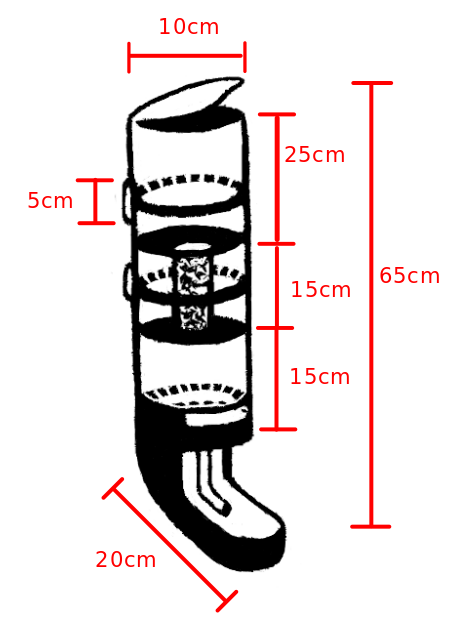
\includegraphics[scale=0.7]{/home/grmunhoz/Documents/Munhoz/University/Pictures/draft2.1.png} 
\label{figetapas}
\legend{Fonte: Autoria Própria}
\end{center}
\end{figure}


O produto possui no total 65 cm de altura e consegue armazenar um pouco mais de 3 litros de água devido seu diâmetro de 10 cm. O bocal possui 7cm de altura e um diâmetro de apenas 1 cm, já o acessório de cantil de água possui 10 cm de altura e 20 cm de comprimento sendo sua largura do mesmo diâmetro do corpo do produto. 

O material predominante no produto é o plástico polipropileno reciclado. Esse termoplástico é utilizado em toda a estrutura do bebedouro, inclusive no bocal e no acessório de cantil. Enquanto o filtro é um conjunto de carvão ativado envolto por plástico também polipropileno. Além desses materiais também se encontram no produto pequenas partes de metal para encaixes e adesivos nos suportes para fixação em superfícies.


\section{Definir ergonomia e estética}

A ergonomia do produto foi pensada tanto para a utilização pelos pets assim como para a manutenção do equipamento pelos tutores. Foi projetado um sistema de suporte de fácil instalação e que pode ser utilizado em diversos tipos de superfícies. Dessa forma se o cliente utiliza um bebedouro elevado, o produto desenvolvido consegue ficar na altura ideal e caso o dono estiver usando o acessório de cantil suspenso os animais não precisam se abaixar muito para beber a água. 
<<<<<<< HEAD

Outro ponto importante abordado em relação a ergonomia foi a manutenção do filtro e o preenchimento com água. A tampa primeiramente possui uma borda lateral que facilita a abertura e o preenchimento com água, já que a tampa pode ser aberta por completo por meio de uma pequena dobradiça. Além disso, o diâmetro do tubo de armazenamento foi projetado para que uma pessoa consiga manusear e desrosquear o filtro de forma simples, facilitando assim o processo de troca que deve ocorrer de 6 em 6 meses. 

O processo de limpeza também foi levado em conta para o desenvolvimento da estética e do formato do aparelho. Pensando nisso, o produto consegue ser desmontado de forma fácil e a limpeza pode ser feita rapidamente.

Com relação a estética final, o produto possui várias possibilidades de cores: azul, cinza, vermelho, verde, branco e preto, no entanto, essas cores são apenas utilizadas nos detalhes do bebedouro como os suportes para o bebedouro em si, o suporte para o filtro interno, as tampas e o acessório de cantil. O formato é cilíndrico e possui as arestas arredondadas. 


\section{Definir parcerias de co-desenvolvimento}

=======

Outro ponto importante abordado em relação a ergonomia foi a manutenção do filtro e o preenchimento com água. A tampa primeiramente possui uma borda lateral que facilita a abertura e o preenchimento com água, já que a tampa pode ser aberta por completo por meio de uma pequena dobradiça. Além disso, o diâmetro do tubo de armazenamento foi projetado para que uma pessoa consiga manusear e desrosquear o filtro de forma simples, facilitando assim o processo de troca que deve ocorrer de 6 em 6 meses. 

O processo de limpeza também foi levado em conta para o desenvolvimento da estética e do formato do aparelho. Pensando nisso, o produto consegue ser desmontado de forma fácil e a limpeza pode ser feita rapidamente.

Com relação a estética final, o produto possui várias possibilidades de cores: azul, cinza, vermelho, verde, branco e preto, no entanto, essas cores são apenas utilizadas nos detalhes do bebedouro como os suportes para o bebedouro em si, o suporte para o filtro interno, as tampas e o acessório de cantil. O formato é cilíndrico e possui as arestas arredondadas. 


\section{Definir parcerias de co-desenvolvimento}

>>>>>>> 2428725220ac865e51b23f28ef3236605f1d61ba
Para participar do desenvolvimento do produto foram definidas parcerias no mercado pet, no segmento de termoplásticos e também no setor de embalagens. Entre eles se encontram estabelecimentos varejistas e atacadistas, como pet shops, fabricantes de embalagens e indústrias de injeção plástica. Além disso, também foram negociadas parcerias com canis e ONGs para validação do projeto e também para a divulgação do produto.

%\section{Definir plano macro de processo}

\newpage
\chapter{Projeto Detalhado}
%\pagestyle{fancy}

\section{Criar e detalhar itens e documentos}

No desenvolvimento desta fase, é realizada o descrição em forma de lista dos SSCs (Sistema, Subsistemas e componentes), além da codificação dos produtos, o desenho do mesmo e suas especificações iniciais.

Os SSCs do bebedouro são os seguintes:

\begin{itemize}
\item Sistema: Bebedouro filtrante para PETs
\item Subsistemas: Estrutura externa, adaptadores de bocal, filtro,compartimento secundário e recipiente final
\item Componentes: 
\subitem Estrutura externa: Plástico e apoio
\subitem Adaptadores de bocal: Hastes e garras
\subitem Filtro: Carvão ativado,  Quartzo, Dolomita e Alumina;
\subitem Recipiente: Filete anterior ao recipiente e o próprio recipiente
\end{itemize}

\begin{figure}[H]
\begin{center}
\caption{Detalhamento dos itens}
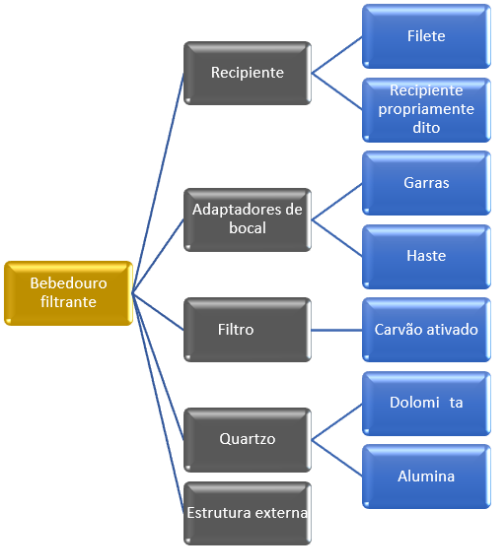
\includegraphics[scale=0.6]{/home/grmunhoz/Documents/Munhoz/University/Pictures/arvore.png} 
\label{figetapas}
\legend{Fonte: Autoria Própria}
\end{center}
\end{figure}

As especificações das tolerâncias são levantadas pelos fornecedores e mantém um padrão considerável e como são poucos componentes com possibilidade de variação está etapa é simples e direta, tendo uma possibilidade de variação no tamanho dos materiais injetáveis em  +/- 0,1 e além disso nenhum tipo de defeito é tolerado, bem como riscos, manchas e raspões.

\section{Decidir fazer ou comprar SSCs}

Para o desenvolvimento do produto, será necessário comprar os componentes como o plástico pronto para realizar a injeção, os componentes do filtro(Carvão ativado,  Quartzo, Dolomita e Alumina), e as hastes de ferro. Com isso, será feito internamente na fábrica a injeção plástica para a produção da estrutura externa do bebedouro, a estrutura do filtro e o recipiente final.

\begin{itemize}
\item Estrutura externa: Plástico e apoio (Fabricar)
\item Adaptadores de bocal: Hastes e garras (Comprar)
\item Filtro: Carvão ativado,  Quartzo, Dolomita e Alumina (Comprar)
\item Recipiente: Filete anterior ao recipiente e o próprio recipiente (Fabricar)
\end{itemize}


\section{Planejar processo de fabricação e montagem}

Os processos de fabricação macro são os seguintes:

\begin{itemize}
\item Injeção plástica da estrutura externa do bebedouro;
\item Injeção plástica da estrutura do filtro;
\item Injeção plástica do recipiente final do bebedouro;
\item Montagem de todas as partes separadas do bebedouro: Recipiente, Filtro, estrutura externa e adaptadores
\end{itemize} 
	
Para a injeção, o procedimento é simples, pois é utilizada um mesmo modelo de máquina injetora com moldes diferentes para cada tipo de injeção(recipiente e estruturas externas);

Para a montagem o procedimento será o seguinte:
\begin{figure}[H]
\begin{center}
\caption{Processo de montagem}
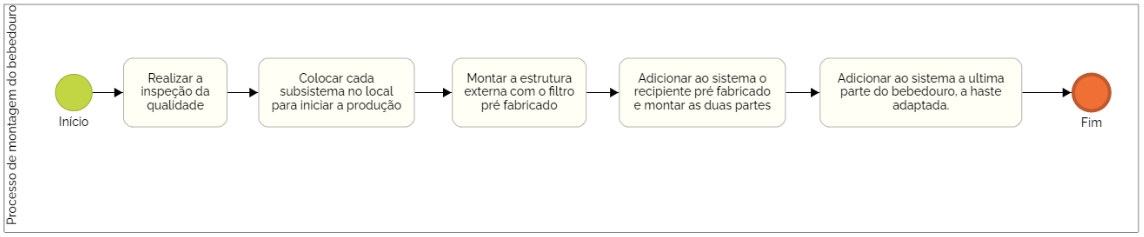
\includegraphics[scale=0.5]{/home/grmunhoz/Documents/Munhoz/University/Pictures/processo.png} 
\label{figetapas}
\legend{Fonte: Autoria Própria}
\end{center}
\end{figure}

\section{Projetar recursos de fabricação}

Já os insumos necessários para o o será fabricado internamente na indústria, como comentado anteriormente, são o plástico injetável e a matéria prima para a produção do filtro. 

Para a injeção, algumas matérias primas específicas são necessárias, e para isso existem muitas possibilidades:

\begin{itemize}
\item Injeção de plástico em ABS
\item Injeção de plástico em Nylon
\item Injeção de plástico em Poliestireno
\item Injeção de plástico em Polietileno
\item Injeção de plástico em Polipropileno
\item Injeção de plástico em Poliuretano
\item Injeção de plástico em PVC
\end{itemize}

No entanto, para a produção do produto só serão utilizados alguns desses tipos de injeção.

Os plástico para serem injetados necessitam estar em pedaços, para assim serem colocados nas máquina e assim a injeção aconteça de forma efetiva. a seguir será apresentado em imagem como são os plásticos antes de serem injetados:

\begin{figure}[H]
\begin{center}
\caption{Plásticos para injeção}
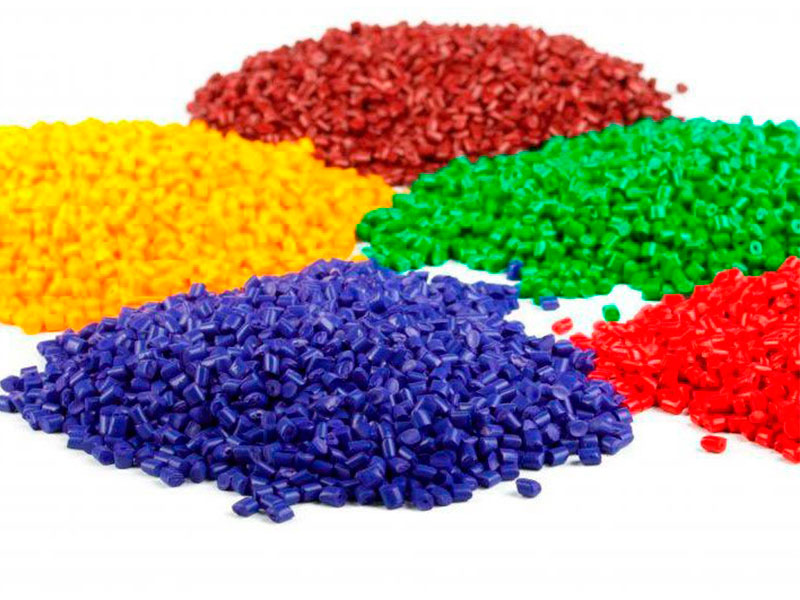
\includegraphics[scale=0.3]{/home/grmunhoz/Documents/Munhoz/University/Pictures/plastico.jpg} 
\label{figetapas}
\legend{Fonte: Google}
\end{center}
\end{figure}


\section{Avaliar itens e documentos}

Para um produto entrar em circulação e poder ser comercializado livremente é necessário estar em consonância com as normas estabelecidas por lei.

Para um produto como um bebedouro, todas as normas estabelecidas foram levadas em consideração desde o início do desenvolvimento do projeto e o produto está dentro de todas as normas existentes.


\section{Otimizar produto e processo}

Como evidenciado no tópico anterior a conformidade com todas as normas vigentes tanto de produção, quanto de utilização, tipo de consumidor, materiais e descarte; foram tomadas como pré-requisitos para o desenvolvimento do produto.

Assim, após a verificação anterior podemos constatar que o produto atende a todas as exigências normativas referentes a sua fabricação, distribuição e uso. Por isso não foi necessária nenhuma otimização nesse sentido.


\section{Criar material de suporte do produto}

O filtro a ser desenvolvido é um item de utilização simples, por isso não foi necessário o desenvolvimento de materiais de suporte complexos. Todavia junto da embalagem do item será enviado um folheto com instruções básicas de utilização e conservação, assim como descrição do item e informações para que os consumidores façam um descarte correto do produto após o fim da sua vida útil.

As informações de utilização e conservação terão como objetivo informar ao consumidor o uso correto do produto além de ações necessárias para sua conservação durante o ciclo de vida do produto e o bom funcionamento.

O material de suporte também contará com uma breve descrição do produto, partes e materiais que compõem o produto, para que o consumidor entenda o produto e esteja ciente da sua composição.

Além disso, contará com as informações para descarte correto do item, seguindo a missão da empresa de popularizar no Brasil a utilização de materiais alternativos e ecológicos em produtos inovadores.

\section{Projetar embalagem}

A embalagem desenvolvida foi pensada para proteger o produto principalmente de danos mecânicos que podem sofrer ao longo do transporte e possibilitar sua distribuição para todo o país. Por não se tratar de um objeto frágil a embalagem será composta basicamente por uma embalagem de papelão onde o produto será colocado dentro e o espaço vazio dentro da embalagem será preenchido por um material chamado Bio Pack.

O Bio Pack é uma espécie de espuma de origem vegetal que pode ser usada para preencher embalagens e proteger objetos. Com composição 100$\%$ biodegradável, o Bio Pack cumpre a função de proteção (comumente desempenhada pelo plástico-bolha), com a vantagem de não agredir o meio ambiente.

Para comportar o nosso produto a embalagem tem 70cm de comprimento, 30 cm de largura e 20 cm de altura.

\begin{figure}[H]
\begin{center}
\caption{Dimensões da embalagem de papelão}
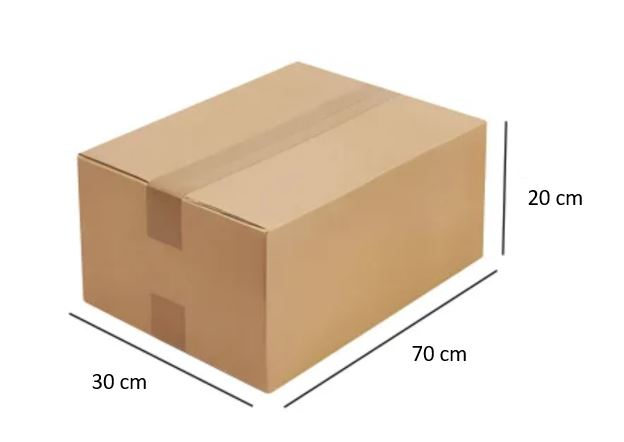
\includegraphics[scale=0.7]{/home/grmunhoz/Documents/Munhoz/University/Pictures/embalagem.JPG} 
\label{figetapas}
\legend{Fonte: Autoria Própria}
\end{center}
\end{figure}

\begin{figure}[H]
\begin{center}
\caption{Bio pack}
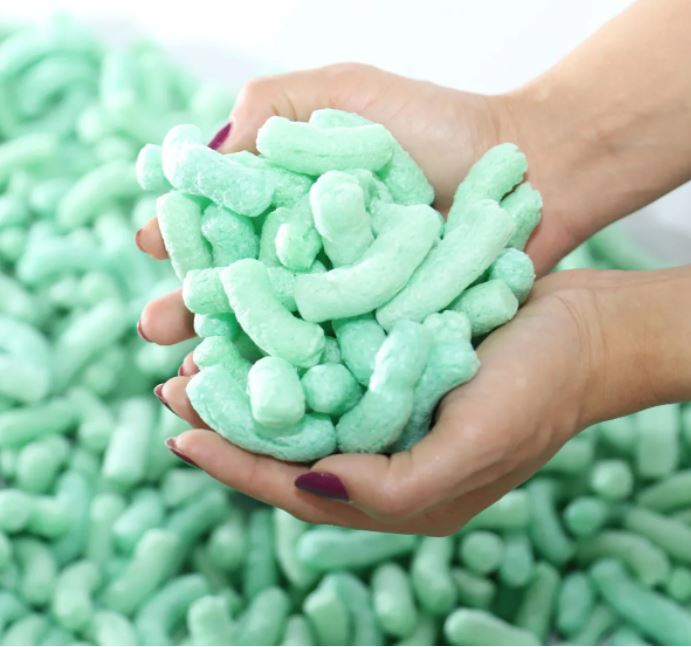
\includegraphics[scale=0.5]{/home/grmunhoz/Documents/Munhoz/University/Pictures/bio pack.JPG} 
\label{figetapas}
\legend{Fonte: Google}
\end{center}
\end{figure}


\section{Planejar fim de vida de produto}

A última etapa do ciclo de vida do produto é justamente o fim da sua vida útil e o descarte ou reutilização. Para nossa empresa o compromisso com o meio ambiente através da reutilização dos produtos ou descarte correto é imprescindível.

Dessa forma para esse produto será disponibilizado ao consumidor um departamento comercial onde a própria empresa receberá de volta o item após o fim da sua vida útil (6 meses) para reutilizar partes dele, já que a empresa conta com um portfólio de produtos ecológicos e reciclados, e também será feito o descarte de produtos que não podem ser reutilizados, como o filtro de carvão ativado.

Caso o consumidor opte por ele mesmo fazer o descarte do material ele deve seguir algumas recomendações. Conforme a Norma Brasileira da ABNT, NBR 10004, os resíduos são classificados nas seguintes classes:

\begin{itemize}
\item Classe I: Perigosos;
\item Classe II: Não perigosos;
\subitem A: Não inertes;
\subitem B: Inertes.
\end{itemize}

O elemento filtrante, que é o carvão ativado, é considerado resíduo Classe II A: Não Inertes. Isso significa que não se apresentam inflamáveis, corrosivos, tóxicos, patogênicos, e nem possuem tendência a sofrer uma reação química. E ainda, podem ter propriedades, tais como: biodegradabilidade, combustibilidade ou solubilidade em água.

Assim, os resíduos que possuem essa classificação podem ser descartados em lixos recicláveis, na lata indicada com a cor vermelha referente a lixo composto por componentes plásticos.

\begin{figure}[H]
\begin{center}
\caption{Lixeira de reciclagem}
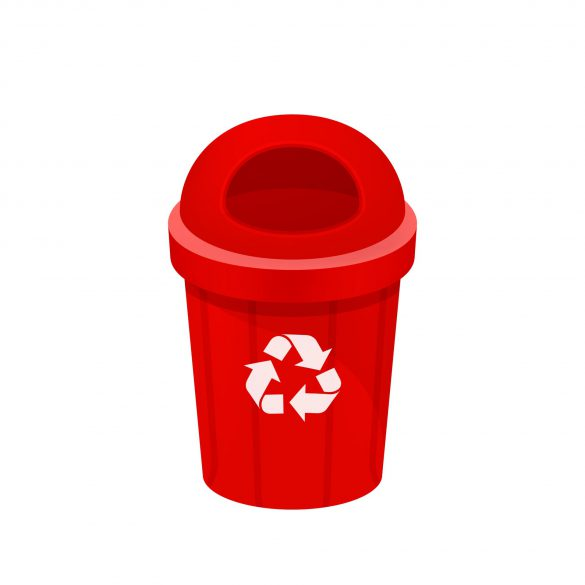
\includegraphics[scale=0.3]{/home/grmunhoz/Documents/Munhoz/University/Pictures/lixeira.JPG} 
\label{figetapas}
\legend{Fonte: Google}
\end{center}
\end{figure}

Além disso, o plástico, material que é feito o corpo do filtro, é reciclável e deve ser descartado em lixeiras específicas para esse material.

\section{Testar e homologar produto}

Após toda a trajetória de desenvolvimento do produto apresentado constatou-se que ele está em conformidade com os objetivos da empresa, sendo viável sua inclusão ao portfólio de produtos, além de se mostrar em conformidade com as necessidades e expectativas dos clientes e principalmente com todas as normas relacionadas.

Além disso, através do protótipo foi possível a realização de testes e comprovado que o item atende a todas as especificações de qualidade do projeto técnico do produto.

Dessa forma o produto está validado e pode ser homologado para iniciar sua fabricação e distribuição ao mercado consumidor.


\newpage
%\chapter{Prototipagem}
%\pagestyle{fancy}


%\newpage
\postextual

\bibliography{referencia}

%\begin{anexosenv}

%\chapter{Código utilizado no software EMSO}

%\begin{lstlisting}
%\end{lstlisting}

%\end{anexosenv}

\end{document}
